\documentclass[../relatorio.tex]{subfiles}
\begin{document}
% - estratégia utilizada
% -- arvore de parsing concreta
% -- classes
% -- hierarquia
% -- descentralização das responsabilidades
% -- diagrama de classes

No âmbito de aplicar as regras da gramática definidas anteriormente,
recorreu-se ao uso do módulo \textit{Yacc} da biblioteca \textit{PLY}. 
Deste modo, constroi-se um \textit{parser}, estabelecendo a análise 
sintática a efetuar.

\subsubsection{Árvore de \textit{Parsing} Concreta}

%árvore de parsing concreta

\subsubsection{Classes}


\begin{figure}
    \centering
    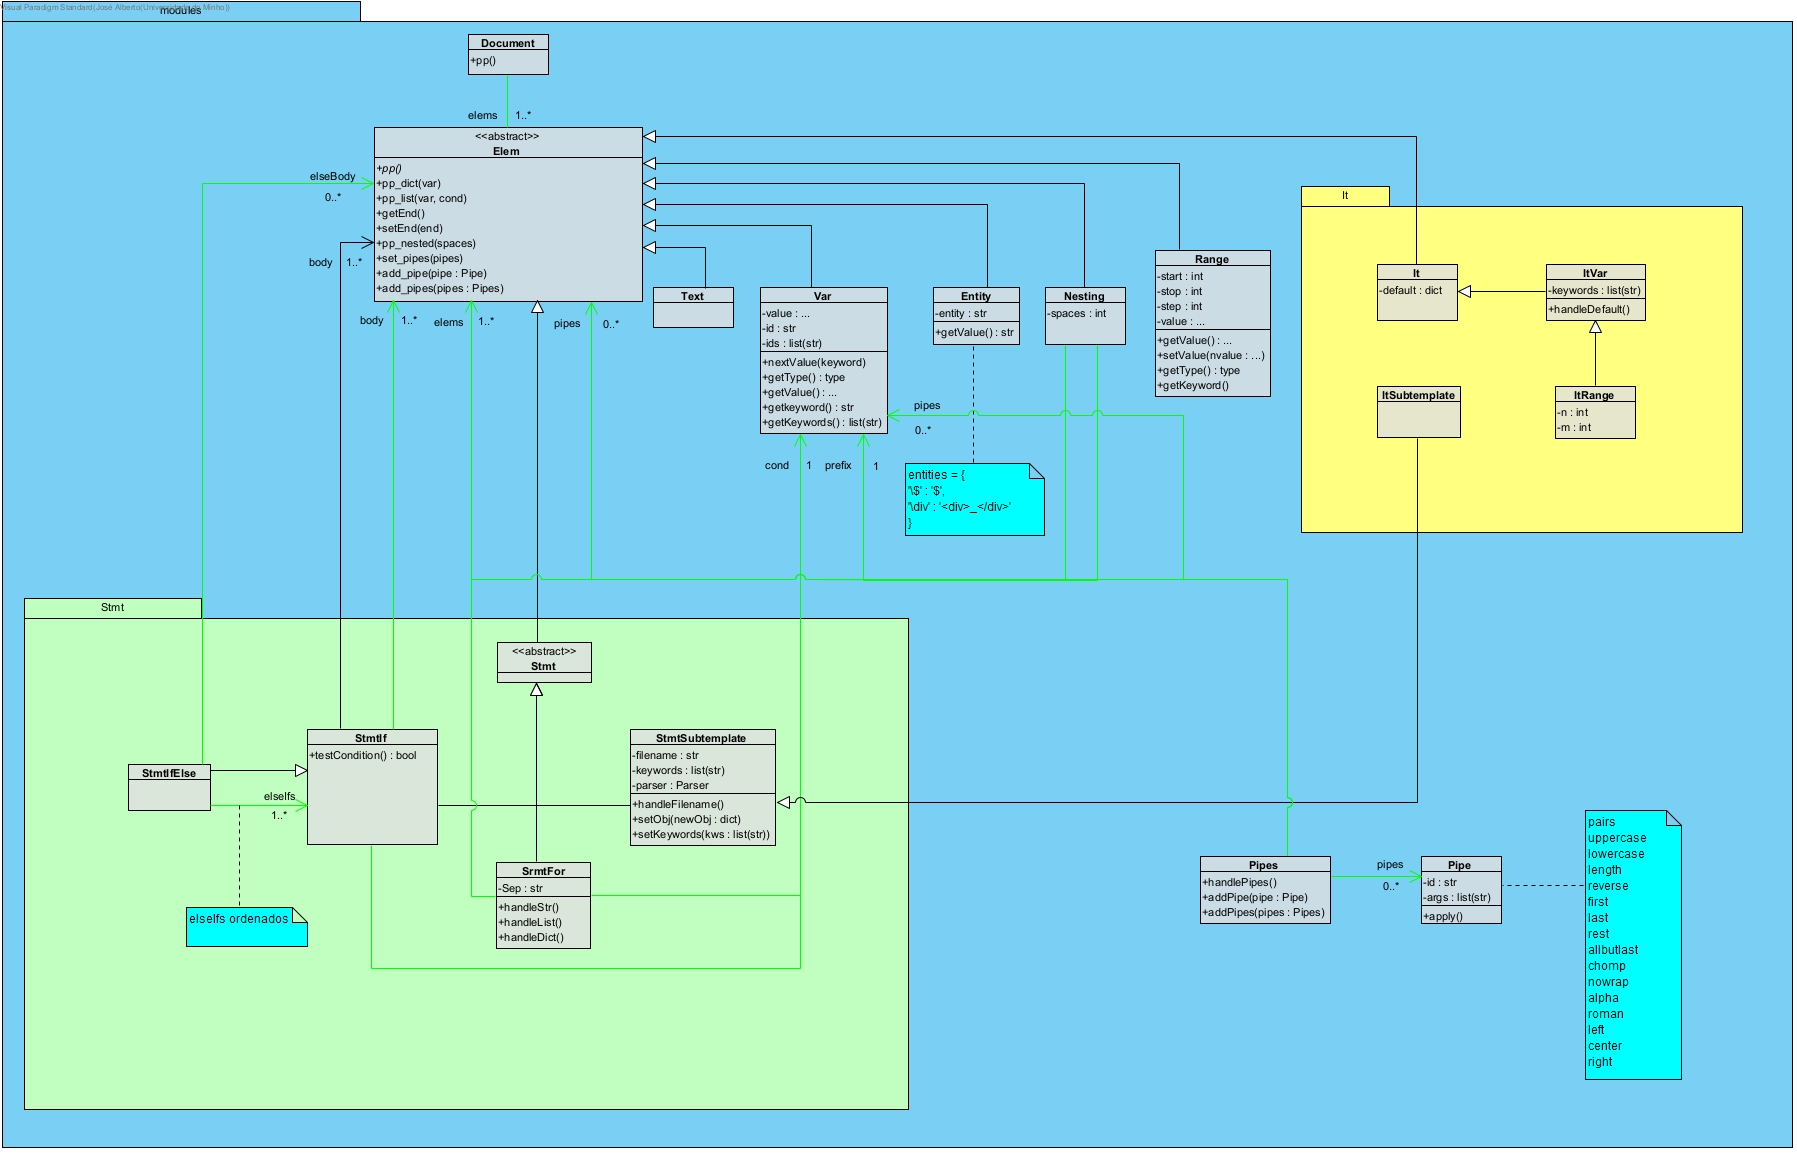
\includegraphics[width=\linewidth]{assets/class_diagram.jpg}
    \caption{Diagrama de classes para os módulos usados.}
    \label{fig:diag_classes}
\end{figure}

\end{document}